%%%%%%%%%%%%%%%%%%%%%%%%%%%%%%%%%%%%%%%%%%%%%%%
%
%   Brief history of TF
%
%%%%%%%%%%%%%%%%%%%%%%%%%%%%%%%%%%%%%%%%%%%%%%%
\section{Data Mining}
\label{sec:2_2_SML}
A closely related field to machine learning is Data Mining, which is defined in \cite{lantz2013} as, "\textit{the generation of novel insights from large databases}". While in \cite{garcia2015}; data mining is defined as, "\textit{solving problems by analyzing data present in real databases}". While others \cite{chakrabarti2006,han2011,nisbet2009,clifton2010} view DM as, "\textit{the main steps of knowledge discovery in databases}". The main distinction between ML and DM is that; ML is dedicated to teach computers how to use data to solve problems, while DM is dedicated to teach computers how to identify patterns like a human to solve problems. It is interesting to mention that every DM involves the use of ML, but not all ML involves DM. Next, a brief description of data mining categories is presented:
 
\begin{itemize}
    \item [-] \textbf{Unsupervised Learning}: Those techniques deal with an unlabeled dataset, with a minimum of human intervention \cite{fisher2014}. Data with no pre-existing labels at our disposal and the purpose is to find associations, relationships, regularities, and similarities in the data. Cluster analysis is among the common models used in unsupervised learning. Cluster analysis is the process to segment/group datasets with shared attributes \cite{kaufman2009}. Unlabeled examples are given an implied cluster label from the relationships within the data entirely. Sometimes, the clustering task is referred to as "unsupervised classification", because it classifies unlabeled examples.   
    
    
\item[-] \textbf{Supervised Learning:}   Supervised learning is popular in the field of DM, commonly knows as prediction methods. In supervised learning, a relationship is to be learned between input space and target space. Based on the predicted target type, there are two common tasks; regression and classification. In regression, the numerical output to be predicted falls in a certain interval. Contrary to classification, the domain of the target is finite and categorical.   
\end{itemize}

    



Next, all the subsequent sections will be dedicated to the classification task in matching with the core of this thesis. In the classification problem, the input attributes (features) and the target attribute (class) are transparent. The aim is to learn a function that maps inputs to outputs. The learned function is called a model, and it is inferred from labeled training data. Let, 

\begin{equation}\label{eq:classification}
\textbf{x}=\left[x^{(1)},..., x^{(d)}\right]^T,\textrm{ and } \textbf{x}\in \mathcal{X}=\mathcal{X}^{(1)}\times ... \times \mathcal{X}^{(d)}
\end{equation}
 
\noindent where $\mathcal{X} $ denotes feature space and \textbf{x} is the sample, i.e., \textbf{x} is the so-called feature vector which informs about attribute values. We will assume that we have $d$ attributes at our disposal. The supervised classification model will assign a given object described by its features, \textbf{x}, into one of the predefined categories, also called labels. Let $\mathcal{M}=\{1,..., M\}$ stands for the set of class labels (decision regions). The classification algorithm (discrimination algorithm) is any learned function $\Psi$ with domain $\mathcal{X}$ and codomain $\mathcal{M}$ as clarified in Equation (\ref{mapper}). Where the target values in codomain are finite and categorical.  

\begin{equation}\label{mapper}
\Psi\: :\: \mathcal{X} \to \mathcal{M}.
\end{equation}

\begin{figure}[!ht]
    \centering
    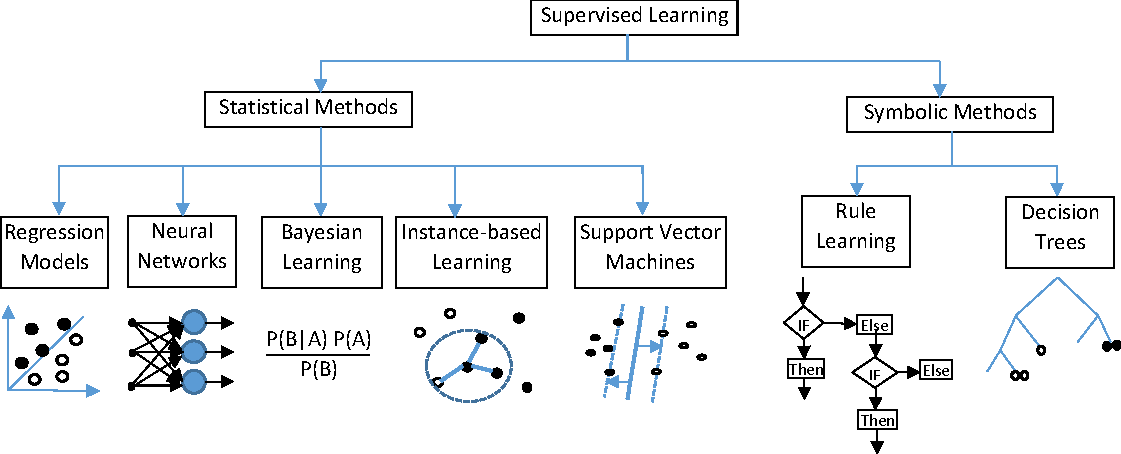
\includegraphics[width=\textwidth]{2_Background/figures/fig_SML_models.pdf}
    \caption{Supervised classification algorithms.}
    \label{ch2:cl.sml}
\end{figure}

There is a large number of models with different inferring strategies to discover the hidden patterns from data. Next, I provide a short review of popular classification algorithms according to the division in Figure \ref{ch2:cl.sml}, inspired by \cite{garcia2015}.  

\begin{itemize}
    \item Regression Models: Logistic Regression (LR) is a statistical model, that returns a probability for each class level. The cutoff value is embedded to separate the upper and the lower probabilities to work as a binary classifier (binomial LR). While multinomial LR deals with more than two classes. In order to be enabled, the missing values should be handled. In addition, the high correlation among the predictors (variables) should be minimized. LR has been praised for its robustness and simplicity \cite{friedman2001}.  \item Artificial Neural Networks (ANNs): The excessive and growing formulations of ANNs from the theoretical and algorithmic depth \cite{carlini2017}, made them more influence on the field of pattern recognition. ANNs handle large and complex tasks due to their nested non-linear structure. While non-explanation is one of the pitfalls of those black-box models.  The computations of those models are based on the definition of neurons. ANNs are unstable and more sensitive to small changes in training data. Similar to LR, they require no missing values.  
    \item Bayesian Learning: Based on the probability theory to get rational decisions \cite{saritas2019}. The Na\"ive Bayes is the most popular algorithm in this category. The posterior probability for each class label is calculated, then the decision is promoted upon the maximum probability returned. Those methods only work with categorical attributes, cannot work with missing values, and are very sensitive to redundancy. The "Na\"ivety" comes from the assumption of the conditional independence between features. It can be viewed as an explainable model to give reasoning about the decisions. 
    \item Instance-based Learning: The prediction of a new unknown sample is based on a distance function with the past stored samples. Also called memorization techniques and lazy learners \cite{lopes2015}. The performance of those methods is affected by the used distance function, neighborhood size, and decision aggregation mechanism. K-Nearest Neighbor (KNN) is the most popular method in this category. Pitfalls of those methods can be mentioned as: high memory space for storage, delayed prediction response, sensitivity to noise.
    \item Support Vector Machines (SVM): Learning algorithms which are based on maximizing gab separation (margin) between different class samples to get correct decisions. They are suitable to work as linear and non-linear data separation. Only the class borders (support vectors) are important to optimize the margin where internal points can be removed to improve the efficiency \cite{nalepa2019}. They require no missing values and are commonly robust against noise. \item Rule Learning: Called divide-conquer algorithms \cite{furnkranz2012}. The data parts are divided based on one rule, then recursively conquer the divided parts. Those models are transparent or explainable to nonexperts in the form of logical structures. Available features are analyzed to find homogeneous groups, then an additional rule is built to drill down more. Small changes in the training data results in decision change. Rule learning techniques are affected by missing values, noisy samples, and outliers.
    \item Decision Trees (DT): This is a kind of indirect rule learning. Uses structure branching decisions to model the relationships among the features and the predicted class value. They are widely used and can model any type of data. The human-readable model is appropriate in applications where legal reasoning is required. Those models are vulnerable to overfitting, and the internal parameters should be tuned \cite{geron2019}. Unstable like ANNs and sensitive to change in the training data. Usually, they are biased towards the splits on features.               
\end{itemize}

For unseen pattern $\textbf{x}$, a class membership values are calculated as in Equation (\ref{membership}), then the labeling choice will be connected to the highest score.
\begin{equation}\label{membership}
\Psi(\textbf{x})=\text{Max}\{g_1(\textbf{x}),g_2(\textbf{x}),\dots,g_M(\textbf{x})\}
\end{equation}


 The decision region $R_1$ for the $1^{st}$ class, is the set of points for which $g_1(\textbf{x})$ has the highest score \cite{kuncheva2014}. While the \textit{classification boundaries} contain data points for which the membership values tie. If the decision region $R_1$ contains data points from the $2^{nd}$ class, then we have overlapped classes. From Figure \ref{ch2:overlapping}. (c) and as shown in \cite{galbusera2019}, the regions are nonoverlapping as the model learns all the details about the data. This case is known as overfitting, and the model will not perform properly to predict unseen samples. While  Figure \ref{ch2:overlapping}. (a) shows the optimal class separation boundary that guarantees minimum possible error with the future samples. Finally,  Figure \ref{ch2:overlapping}. (b) shows the the underfitting case when the model fails to capture relationships between a dataset’s features and a target variable during training. 
 
 
 \begin{figure}[!ht]
    \centering
    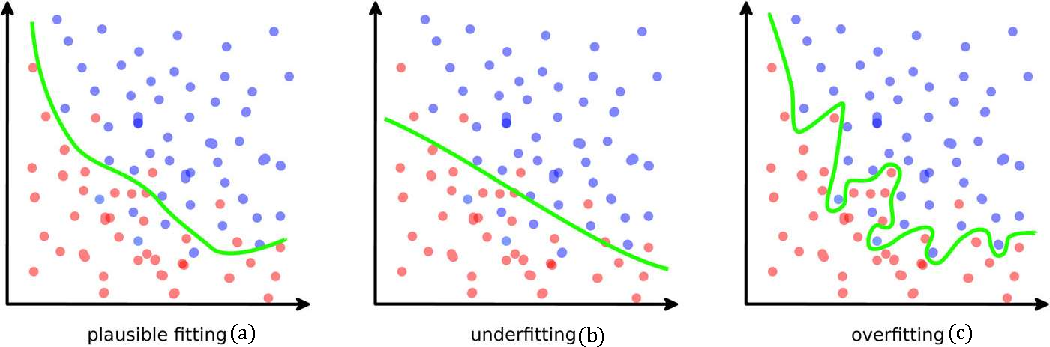
\includegraphics[width=\textwidth]{2_Background/figures/fig_overlapping.pdf}
    \caption{Trade-off between overlapping and overfitting, taken from \cite{galbusera2019}.}
    \label{ch2:overlapping}
\end{figure}


Each model has an accompanied error, we need to understand the different sources that cause this error. Equation (\ref{Gen.error}) represents the compound generalization error $E_G$ of a classifier $\Psi$ that is trained on dataset $D$. 


\begin{equation}\label{Gen.error}
E_G(\Psi,D)=E_A(D)+ E_M+E_B
\end{equation}

\noindent where $E_A(D)$ is the "approximation error" represents the variance due to using different training data, or non-deterministic training algorithm. Clarified as, the hyper-parameters of the model that affect its performance. The second term $E_M$ is the "model error" which represents the bias due to selecting a model in preference of another. The last term $E_B$ is the "irreducible error" coming from the insufficient representation of the data. This is commonly known as Bias/Variance Tradeoff \cite{geron2019,kuncheva2014}. Increasing a model’s complexity will typically increase its variance and reduce its bias.
Conversely, reducing a model’s complexity increases its bias and reduces its variance.
This is why it is called a tradeoff.    